\chapter{Interactive Map Labeling}
\label{chapter:map_annotation}

World representation of robots should enable effortless communication between users and robots. Robots that co-exist with humans will need to accept commands from human users. As mentioned in Chapter \ref{chapter:introduction}, the robot keeps a metric map for autonomous navigation. Requiring users to understand the robot's internal representation of the world and to provide goals in terms of metric coordinates may not be a convenient way of interaction. For example, it is not easy for someone to quickly interpret the floor plan and provide a goal with explicit coordinates $(1.2,4.5,0.0)$. Maps should include spatial information to support tasks that requires more than simple obstacle avoidance. For example, if the task involves interaction with planar surfaces, landmarks, objects, or people; a robot's map should be able to represent these information. For these reasons, adding semantic information to robot maps is essential. There are several methods to support the annotation of entities in a robot map. For example, while the robot is building its representation of the environment, it can recognize objects or landmarks such as doors, tables, rooms and automatically add these features to its map. Even though such a system would be useful, it may wrongly label some objects. In that case, the correct label can be provided by a human with an interactive system. Custom labels would also allow unique annotations such as \textit{"John's Room"}.

We use a map representation that includes 2D waypoints, 3D polygons that defines the boundary of planar surfaces and objects along with user-appointed labels. We give more details about waypoint representations in Section \ref{sec:map_waypoints}, planar surfaces in Section \ref{sec:map_landmarks} and objects in Section \ref{sec:map_objects}. To add labeled landmarks and objects to the semantic map, we use an interactive system that uses a combination of a graphical user interface (GUI) and natural pointing gestures. Using the GUI, users can command the robot to follow them, add waypoints along the robot's path and add landmarks or objects to the map by pointing at them and entering a label. Our GUI is shown in Section \ref{sec:map_ui} and our approach to determine the pointing gesture targets is presented in Section \ref{sec:pointing_gestures}.

\section{Related Work}
\label{sec:map_relevant_work}

One of the key concepts in semantic mapping is establishing a \textit{common ground} \cite{clark1991grounding}. By referring to same structures and objects with the same reference, the communication about labeled entities is grounded.

One of the closely related works to our interactive labeling approach Human Augmented Mapping, introduced by Topp and Christensen in \cite{topp2006topological} and \cite{topp2010detecting}. This approach involves labeling two types of entities: regions and locations. Regions are meant to represent areas such as rooms and hallways, and serve as containers for locations. Locations are meant to represent specific important places in the environment, such as a position at which a robot should perform a task. This approach was applied to the Cosy Explorer system, described in \cite{zender2007integrated}, which includes a metric map, a topological map, as well as detected objects. While our goal is similar, we use a different map representation, method of labeling and interaction design. Kuipers \cite{kuipers2000spatial} introduced Spatial Semantic Hierarchy, which is a method of organizing semantic information for spatial regions. Another application using semantic maps is direction following, studied by Kollar \cite{kollar2010toward}. This work describes a system capable of following directions in natural language, i.e. ``go past the computers". People also routinely use semantic relationship of objects when they refer to objects. For example, the robot can handle a command such as ``get the mug on the table".

\section{Semantic Maps}
\label{sec:map_semantic_maps}

Semantic mapping aims to create maps that include various types of semantic information to allow the robot to have a richer representation of the environment. In this section, we briefly present the semantic information we use to enrich the occupancy grid maps: waypoints, planar landmarks and objects. Although we describe three types of entities for storing semantic information, it is possible to include more features.

\subsection{Navigation Waypoints}
\label{sec:map_waypoints}

We define navigation waypoint as a navigable pose represented in the map frame. A pose $(x,y,\theta)$ represents the position and orientation of with respect to a coordinate frame. We will refer a navigation waypoint simply as a waypoint for the remainder of this text. Using the GUI, a user can save the robot's current pose along with a label, assuming that the robot is properly localized in the map. This method is the most straightforward way to save a pose and use it later for a task. When the robot is asked to navigate to a labeled waypoint, the goal of the robot is simply the saved pose.

Even though the waypoint method is easy to use and practical, it has shortcomings. It fails to capture the shape and extent of the structure designated by the label, which might be important for some tasks, such as object search. Moreover, point based references may be ambiguous to represent a region or volume in a map, such as a hallway or a room. For example, if the user wants to save hallway as a landmark, it is useful to have a representation of the location and the extent of the hallway. Another example is that the user can label a coffee table, which is a movable object. Instead of saving a fixed coordinate location for the landmark, robot can save the planar surface and can potentially have a model to handle moving landmarks. This gives the robot robustness in its operations and a method to potentially use the planar surfaces as features in localization \cite{trevor2012planar}.

\subsection{Planar Surfaces}
\label{sec:map_landmarks}

In this type of semantic information, we keep track of a set of observed planar surfaces as part of the map representation. We use a front-facing RGB-D camera to acquire suitable data. Planes are extracted from the point cloud by an iterative RANdom SAmple Consensus (RANSAC) method, which allows us to find all planes meeting constraints for size and number of inliers. A clustering step is performed on extracted planes to separate multiple coplanar surfaces, such as two tables with the same height, but at different locations. We make use of the Point Cloud Library (PCL) \cite{rusu20113d} for much of our point cloud processing. Planes are represented in the hessian normal form. Since the observed planes do not have infinite extent, we bound the observed area with a polygon - in this case, the convex hull of all the observed points on the plane. The convex hull is accompanied with a user-provided label. 

In order to label a planar landmark, the user goes through the following sequence:

\begin{enumerate}
\item User activates basic person following behavior (Section \ref{sec:following_basic_person_following}) and comes near a planar surface of interest.
\item Robot adjusts its pose so it can perceive both the surface and the user.
\item User enters the label using the GUI and activates pointing gesture recognition
\item User performs a pointing gesture towards the landmarks of interest
\end{enumerate}

The act of labeling a planar surface with a label "Table" from the view of the RGB-D camera planted on the robot is shown in Figure \ref{fig:pointing_table_desk}. After the labeling process, the planar landmark is added to the map representation.

\begin{figure}[ht!]
\centering
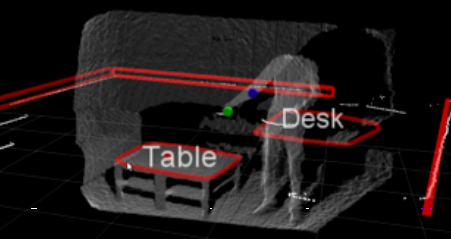
\includegraphics[width=0.55\textwidth]{pics/pointing_table_desk}
\caption{A user is pointing at a table to add it to the semantic map}
\label{fig:pointing_table_desk}
\end{figure}

\subsection{Objects}
\label{sec:map_objects}

Our approach allows interactively building object models for selected objects, and then annotate these models with a label. This enables the robot to quickly build a small object database of the specific objects it needs to interact with. The interactive system works as described in the previous section. Different from labeling planar landmarks, however, we keep a bag of features for each object in the database. Once a user has performed a pointing gesture to label objects, the robot moves to a favorable position and activates its its pan-tilt unit to aim the sensors at this location. Object segmentation is performed using point cloud data from an RGB-D sensor. First, the large planar surface corresponding to the table is detected. This is removed from the point cloud, and point clusters above this are detected. The robot calculates the likelihood of each object being the target, as will be explained in Section \ref{sec:pointing_gestures} and confirms with user if ambiguity is detected. After the target is confirmed, the cluster points are projected into the camera image, and are used to generate a region of interest. SURF features are found in the region of interest, and are stored as an object model along with the provided label.

\section{Graphical User Interface}
\label{sec:map_ui}

We developed an on-board tablet interface to enable interaction between the user and the robot. Similar functionality could be achieved with a speech recognition system, however we think a touch interface is a more robust type of communication. The interface has been implemented on a Nexus 7 Tablet running on Android Operating System. The tablet is equipped with WiFi and talks with the robot using a TCP-based server-client communication model. The client must have the the IP address of the server machine to establish the connection. The messages are sent back-and forth as via XML files. The XML files are serialized and de-serialized using \textit{libXML++} for \textit{C++} (server) and \textit{XMLPullParser} (client) for Android OS. With the tablet interface, a user can do the following:

\begin{itemize}
\item Add/Delete a Labeled or Generic waypoint
\item Label a Planar Surface or Object
\item Initiate Person Following
\item Initiate Person Guidance to a Labeled Planar Surface/Object/Waypoint
\item Stop Robot
\item Change IP Address and Port of the TCP connection
\end{itemize}

A screenshot of our tablet user interface is shown in Figure \ref{fig:ui}.

\begin{figure}[ht!]
\centering
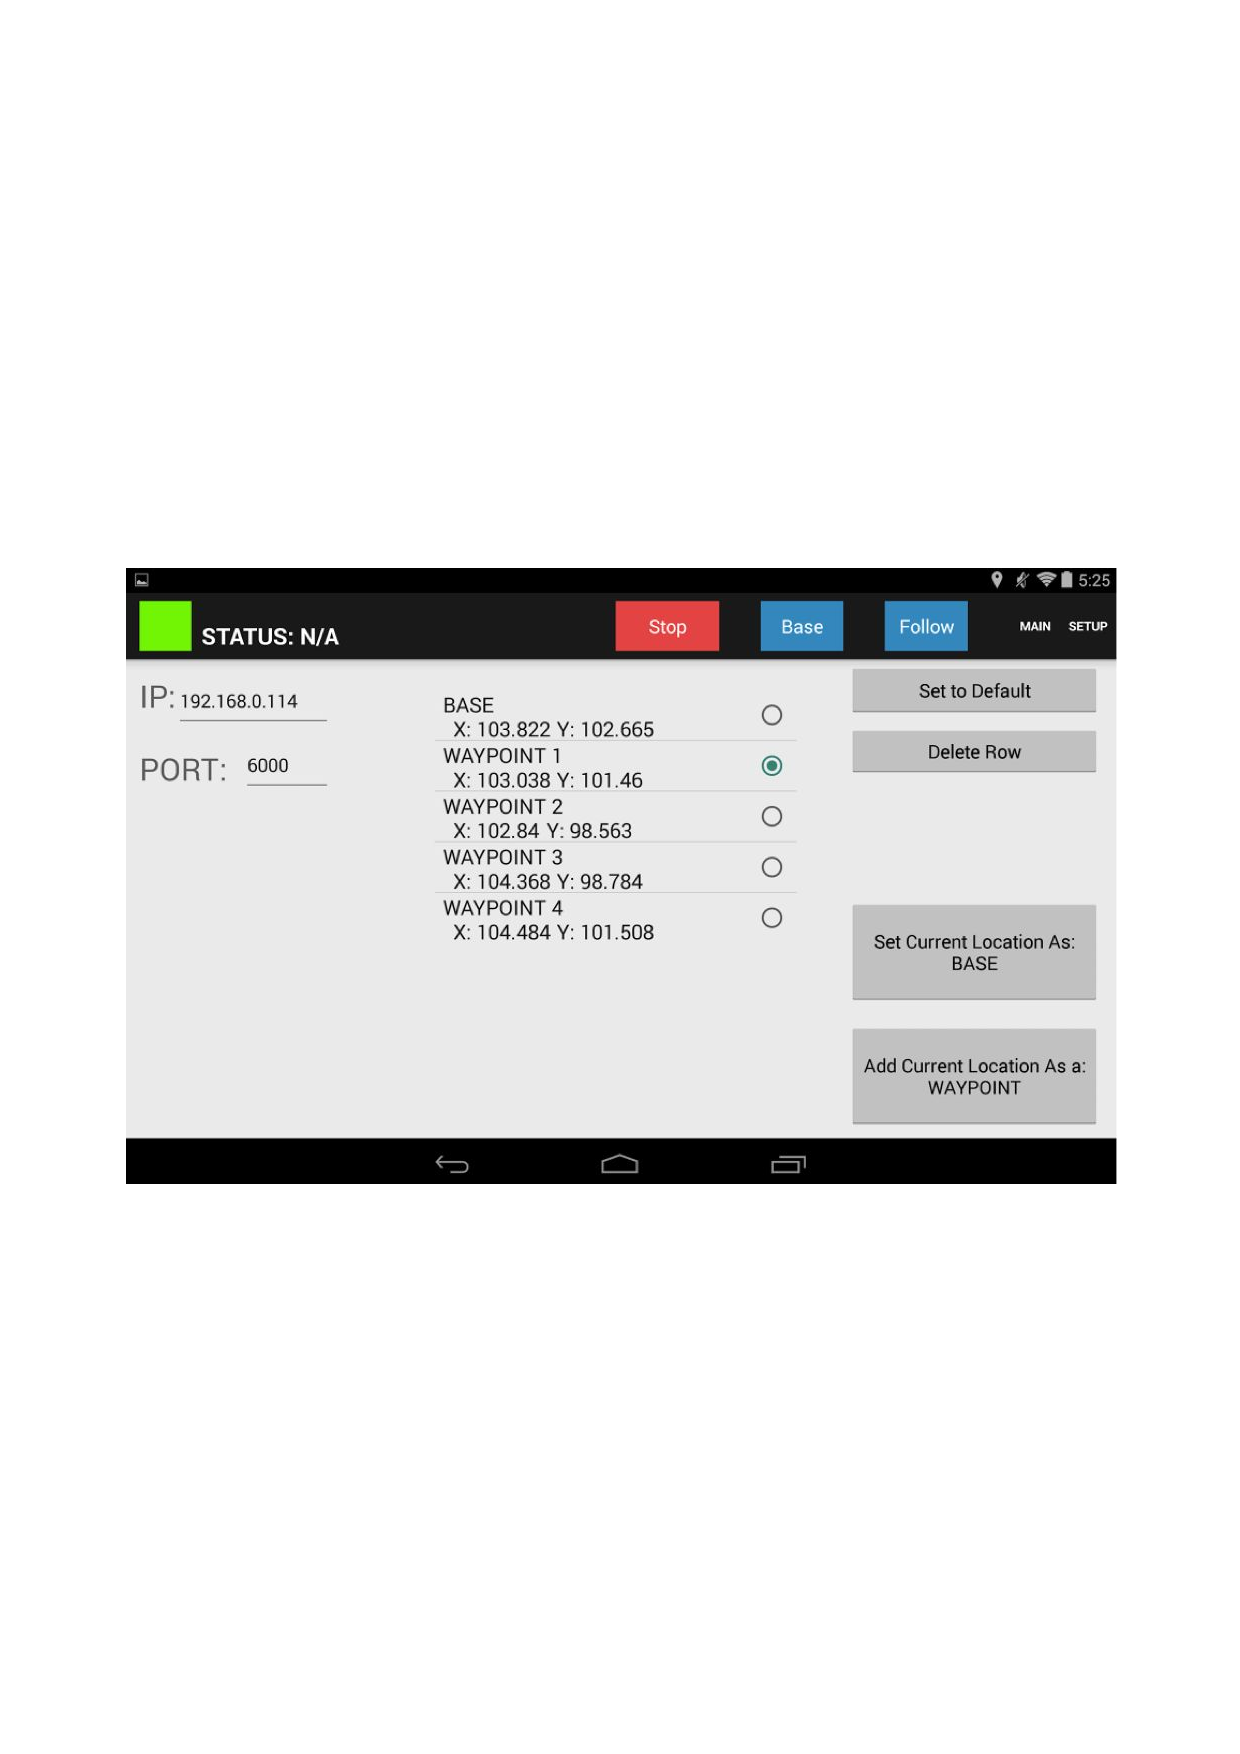
\includegraphics[width=0.75\textwidth]{pics/ui}
\caption{A snapshot from the GUI that runs on robot's touch screen}
\label{fig:ui}
\end{figure}

\section{Pointing Gestures for Human-Robot Interaction}
\label{sec:pointing_gestures}

A natural way to refer to objects and landmarks is to point at them. In this work, we analyze the performance of our pointing gesture recognition, and present an uncertainty model that enables us to reason about ambiguity in pointing gestures, when gesture targets are too close to one another. We model the uncertainty of pointing gestures in a spherical coordinate system, use this model to determine the correct pointing target, and detect when there is ambiguity. Two pointing methods are evaluated using two skeleton tracking algorithms: elbow-hand and head-hand rays, using both OpenNI NITE and Microsoft Kinect SDK~\cite{shotton2011real}.  A data collection with 6 users and 7 pointing targets was performed, and the data was used to model users pointing behavior.  The resulting model was evaluated for its ability to distinguish between potential pointing targets, and to detect when the target is ambiguous.  An example scenario is shown in Figure \ref{fig:cover_pointing_gestures}.

\begin{figure}[ht!]
\centering
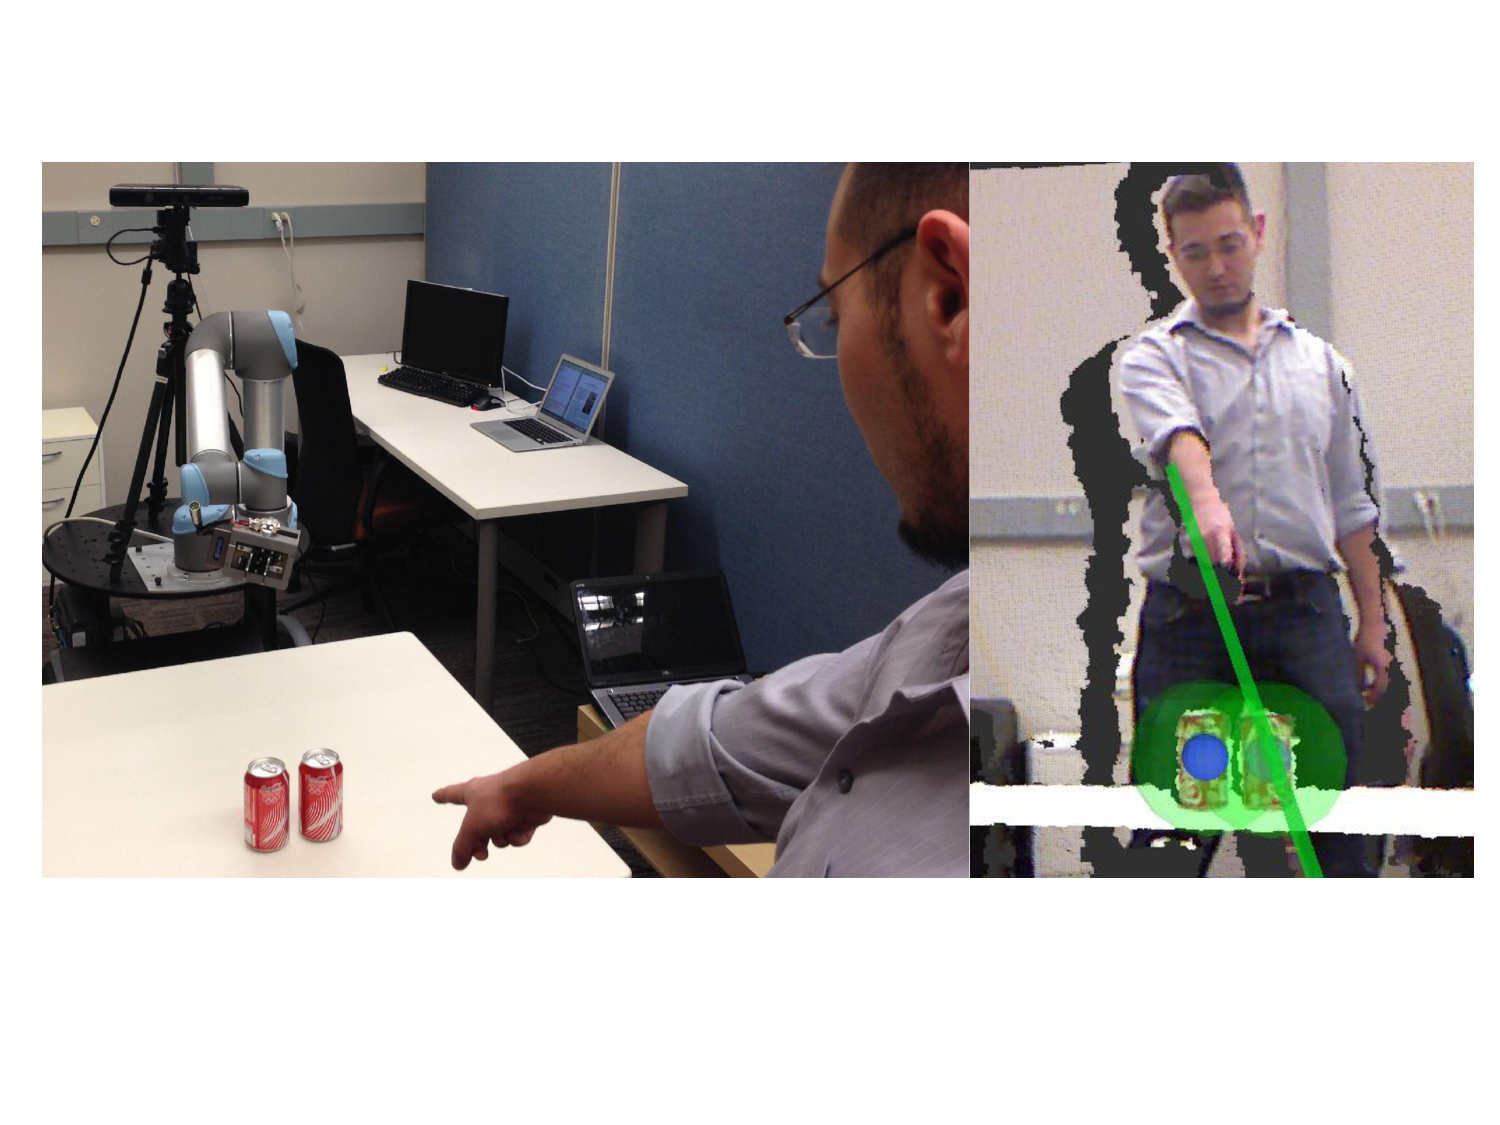
\includegraphics[width=0.8\textwidth]{pics/cover_pointing_gestures}
\caption{(Left) Our approach allows a robot to detect when there is ambiguity on the pointing gesture targets. (Right) The point cloud view from robot's perspective is shown. In this demonstration, both objects are identified as potential intended targets, therefore the robot decides that there is ambiguity.}
\label{fig:cover_pointing_gestures}
\end{figure}

\subsection{Related Works}
\label{sec:pointing_related_works}

Pointing gestures are widely used in Human-Robot Interaction applications. Examples include interpretation of spoken requests~\cite{zukerman2010interpreting}, pick and place tasks~\cite{blodow2011inferring}, joint attention~\cite{droeschel2011towards}, referring to places~\cite{hato2010pointing} or objects~\cite{schmidt2008interacting}, instructing~\cite{martin2010estimation} and providing navigation goals to a robot~\cite{raza2013human}. 

Early works on recognizing pointing gestures using stereo vision utilized background subtraction~\cite{cipolla1996human,jojic2000detection,kahn1995understanding}. Other popular methods include body silhouettes~\cite{kehl2004real}, hand poses~\cite{hu2010hand}, motion analysis~\cite{matikainen2011prop} and Hidden Markov Models~\cite{wilson1999parametric, bennewitz2008robust, li2005hierarchical, nickel2003pointing, droeschel2011learning, aly2012integrated}. Matuszek~\cite{matuszek2014learning} presented a method for detecting deictic gestures given a set of detected tabletop objects, by first segmenting the users hands and computing the most distal point form the user, then applying a Hierarchical Matching Pursuit on these points over time. 

After deciding if a pointing gesture occurred or not, an algorithm must estimate the direction of pointing. This is typically done by extending a ray from one body part to another. Several body part pairs are used in the literature, such as eye-fingertip~\cite{kehl2004real} and shoulder-hand~\cite{hosoya2004arm}; with the two of most commonly used methods being elbow-hand~\cite{raza2013human, brooks2006working, blodow2011inferring} and head-hand~\cite{bennewitz2008robust, schmidt2008interacting} rays. Some studies found that head-hand approach is a more accurate way for estimating pointing direction than elbow-hand~\cite{quintero2013sepo, droeschel2011towards}. Recent works made use of skeleton tracking data  in depth images~\cite{quintero2013sepo, blodow2011inferring, raza2013human}. Other approaches, such as measuring head orientation with a magnetic sensor~\cite{nickel2003pointing} and pointing with a laser pointer~\cite{cheng2009hand, kemp2008point} is reported to have a better estimation accuracy than the body parts method, but require additional hardware. We prefer not to use additional devices in order for the interaction to be as effortless as possible.

Given a pointing direction, several methods have been proposed to determine which target or object is referred by the gesture, including euclidean distance on a planar surface~\cite{cheng2009hand}, ray-to-cluster intersection in point clouds~\cite{blodow2011inferring, quintero2013sepo} and searching a region in interest around the intersection point~\cite{schmidt2008interacting}. Droeschel~\cite{droeschel2011learning} trains a function using head-hand, elbow-hand and shoulder-hand features with Gaussian Process Regression and reports a significant improvement on pointing accuracy. Some efforts fuse speech with pointing gestures for multi-modal Human-Robot Interaction~\cite{aly2012integrated,kowadlo2010influence}. Aly~\cite{aly2012integrated} focuses on relation between non-verbal arm gestures and para-verbal communication based on a HMM approach.

To our knowledge, only Zukerman~\cite{zukerman2011speaking} and Kowadlo~\cite{kowadlo2010influence} considered a probabilistic model for determining the referred object for a pointing gesture. In their approach, the probability that the user intended an object is calculated using the 2D distance to the object and the occlusion factor. Objects that reside in a Gaussian cone emanating from the user's hand are considered as candidates in the model. The approach is implemented in~\cite{zukerman2011speaking}, where it is reported that due to high variance of the gesture recognition system, the Gaussian cone typically encompassed about five objects in cluttered settings. Our work addresses the confusion in such settings. In contrast to their work, we measure Mahalanobis distances to potential target objects using a prior error analysis.

\subsection{Pointing Gesture Representation}

\subsubsection{Pointing Gesture Recognition}
\label{sec:pointing_pointing_gesture_recognition}

Our approach to pointing gesture recognition is to use a third party skeleton tracking package as implemented by OpenNI NITE 1.5 (OpenNI) or Microsoft Kinect SDK 1.5 (MS-SDK). Skeleton tracking software produces 3D positions for several important points and joint positions on the user's body, including hands, elbows, shoulders and head. We use the user's hands, elbows, and head for the recognition of pointing gestures. We are primarily interested in deictic gestures generated by pointing with one's arm. We consider two rays for determining the pointing direction: elbow-hand and head-hand. Both of these methods were evaluated with the two skeleton tracking implementations. For each depth frame, this yields two rays for each of the OpenNI and MS-SDK trackers:

\begin{itemize}
\item{$\vec{v}_{eh} := \vec{p_{elbow}p_{hand}}$}
\item{$\vec{v}_{hh} := \vec{p_{head}p_{hand}}$}
\end{itemize}


When a pointing gesture recognition request is received from a higher level process, the gesture is searched in a time window of \emph{T} seconds. Two conditions must be met to trigger a pointing gesture:

\begin{itemize}
  \item $\vec{v}_{eh}$ makes an angle more than $\phi_{g}$ with the vertical axis
  \item $p_{elbow}$ and $p_{hand}$ stays near-constant for duration $\Delta t_{g}$
\end{itemize}

The first condition requires the arm of the person to be extended away from his/her body, while the second ensures that the gesture is consistent for some time period. The parameters are empirically determined as: $\emph{T}=30s$, $\phi_{g}=45^{\circ}$ and $\Delta t_{g}=0.5s$.

\subsubsection{Representing Pointing Directions}
\label{sec:pointing_representing_pointing_directions}

We represent a pointing ray in two angles: a ``horizontal'' / ``azimuth'' sense we denote as $\theta$ and a ``vertical'' / ``altitude'' sense we denote as $\psi$. We first attach a coordinate frame to the hand point, with its z-axis oriented in either Elbow-hand $\vec{v}_{eh}$ or Head-Hand $\vec{v}_{hh}$ directions, depending on which method is used. The hand point was chosen as the origin for this coordinate system because both of head-hand and elbow-hand pointing methods include the user's hand. The transformation between the sensor frame and the hand frame $^{sensor}T_{hand}$ is calculated by using an angle-axis rotation. An illustration of the hand coordinate frame for Elbow-Hand method and corresponding angles are shown graphically in Figure \ref{fig:pointing_angle_errors}.

\begin{figure}[ht!]
\centering
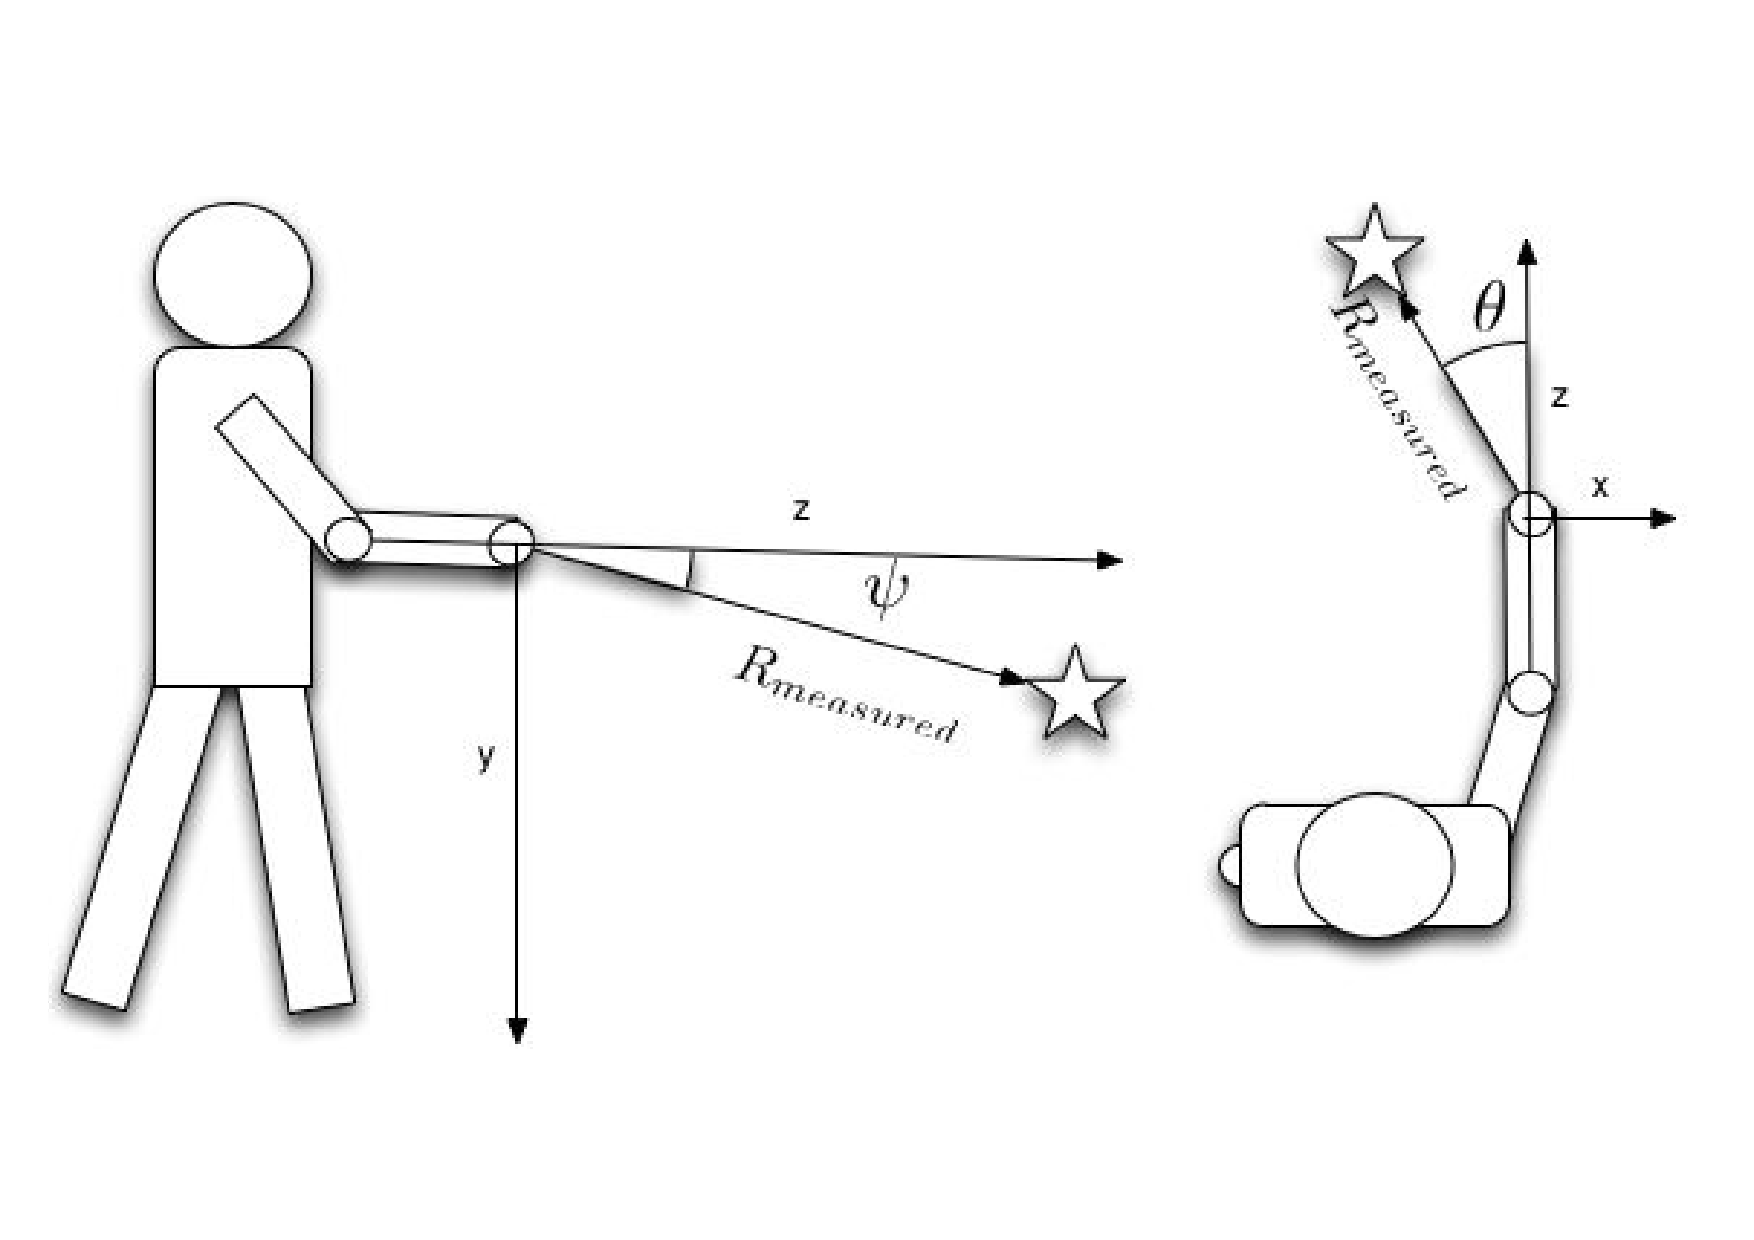
\includegraphics[width=0.8\textwidth]{pics/person_angles_combined_2}
\caption{Vertical $(\psi)$ and horizontal $(\theta)$ angles in spherical coordinates are illustrated. A potential intended target is shown as a star. The z-axis of the hand coordinate frame is defined by either the Elbow-Hand (this example) or Head-Hand ray.}
\label{fig:pointing_angle_errors}
\end{figure}

Given this coordinate frame and a potential target point P, we first transform it to the hand frame by:
$$^{hand}p_{target} = T_{hand} * p_{target}$$

We calculate the horizontal and vertical angles for a target point as $^{hand}p_{target} = (x_{targ}, y_{targ}, z_{targ})$ follows:
$$[\theta_{target}\;\psi_{target}]=[atan2(x_{targ}, z_{targ})\;atan2(y_{targ}, z_{targ})]$$

Where $atan2(y,x)$ is a function returns the value of the angle $\arctan(\frac{y}{x})$ with the correct sign. This representation allows us to calculate the angular errors in our error analysis experiments in Section \ref{sec:pointing_error_analysis}. The angles for each object is then used to find the intended target, as explained in the following section.


\subsubsection{Determining Intended Target}
\label{sec:pointing_determining_intended_target}

We propose a probabilistic approach to determine the referred target by using statistical data from previous pointing gesture observations. We observed that head-hand and elbow-hand methods, implemented using two skeleton trackers, returned different angular errors in spherical coordinates. Our approach relies on learning statistics of each of these approaches, and compensating for the error when the target object is searched for. First, given a set of prior pointing observations, we calculate the mean and variance of the vertical and horizontal angle errors for each pointing method. This analysis will be presented in Section \ref{sec:pointing_error_analysis}. Given an input gesture, we apply correction to the pointing direction and find the Mahalanobis distance to each object in the scene.

When a pointing gesture is recognized, and the angle pair $$[\theta_{target}\;\psi_{target}]$$ is found as described in the previous section, we first apply a correction by subtracting the mean terms from measured angles:
$$[\theta_{cor}\;\;\psi_{cor}]=[\theta_{target}-\mu_{\theta}\;\;\;\psi_{target}-\mu_{\psi}]$$
 
We also compute a covariance matrix for angle errors in this spherical coordinate system: 
$$S_{type} = \begin{bmatrix}
\sigma_{\theta}&0\\ 0&\sigma_{\psi}
\end{bmatrix} $$

We get the values for $\mu_{\theta}, \mu_{\psi}, \sigma_{\theta} ,\sigma_{\psi}$ from Tables \ref{table:pointing_horizontal} and \ref{table:pointing_vertical} for the corresponding gesture type and target. We then compute the mahalanobis distance to the target by:
$$D_{mah}(target,method)=\sqrt{ [\theta_{cor}\;\psi_{cor}]^T S_{method}^{-1} [\theta_{cor}\;\psi_{cor}]}$$
 
We use $D_{mah}$ to estimate which target or object is intended. We consider two use cases: the objects are represented as a 3D point or a point cloud. For point targets, we first filter out targets that have a Mahalanobis distance larger than a threshold $D_{mah} > D_{thresh}$. If none of the targets has a $D_{mah}$ lower than the threshold, then we say the user did not point to any targets. If there are multiple targets that has $D_{mah} <= D_{thresh}$ , then we determine ambiguity by employing a ratio test. The ratio of the least $D_{mah}$ and the second-least $D_{mah}$ among all targets is compared with a threshold to determine if there is ambiguity. If the ratio is higher than a threshold, then the robot can ask the person to resolve the ambiguity.

If the target objects are represented as a point cloud, we then compute the horizontal and vertical angles for every point in the point cloud and find the minimum mahalanobis distance among all. The distance to an object is then represented by this minimum value. Usage of the point cloud instead of the centroid for determining the intended object has several advantages. First, it yields better estimations due to the coverage of the full point cloud. Second, it takes into account the size of the object. For example, if a person is pointing to a chair or door, it is very unlikely that he/she will target the exact center. If the point cloud is used, then we can easily tell that the object is targeted.

 
\subsection{Data Collection}
\label{sec:pointing_data_collection}

To evaluate the accuracy of pointing gestures, we created a test environment with 7 targets placed on planar surfaces in view of a Kinect sensor (Figure \ref{fig:ground_truth_targets}). Depth data was collected from six users, who pointed at each of the seven targets with their right arm while standing at 2 meters away from the sensor. Targets 1 through 4 were on tables positioned around the user, while targets 5 through 7 were located on a wall to the user's right. Our use case is on a mobile robot platform capable of positioning itself relative to the user.  For this reason, we can assume that the user is always centered in the image, as the robot can easily rotate to face the user and can position itself at a desired distance from the user.

\begin{figure}[ht!]
\centering
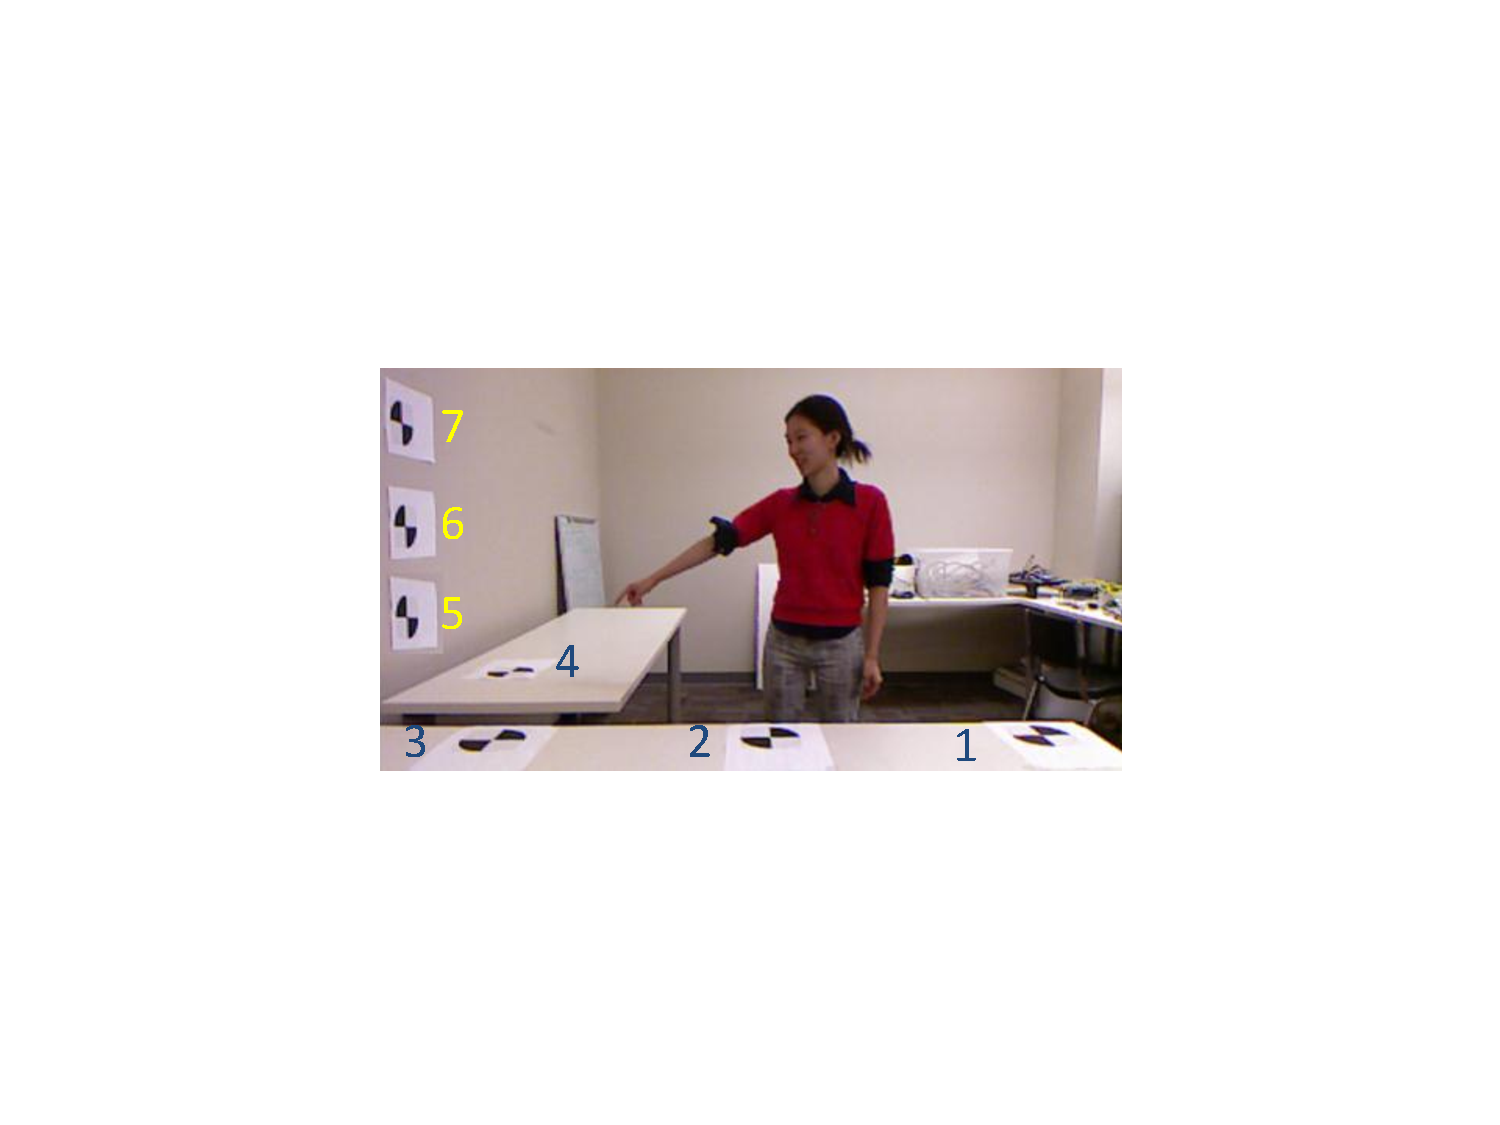
\includegraphics[width=0.65\textwidth]{pics/data_collection_crop}
\caption{Our study involved 6 users that pointed to 7 targets while being recorded using 30 frames per target.}
\label{fig:ground_truth_targets}
\end{figure}

\subsubsection{Ground Truth Target Positions}
\label{sec:ground_truth_points}

We make use of a plane extraction technique from a point cloud to have an accurate ground truth measurement. First, the two table and wall planes are extracted from the point cloud data using the planar segmentation technique described in \cite{trevor2013segmentation}. We then find the pixel coordinates of corners on targets in RGB images, using Harris corner detection \cite{harris1988combined}, which produces calculated corners in image coordinates with sub-pixel accuracy. The pixel coordinate corresponding to each target defines a ray in 3D space relative to the Kinect's RGB camera frame. These rays are then intersected with the planes detected from the depth data, yielding the 3D coordinates of the targets.



%\subsection{Skeleton Data Capture}
%\label{sec:pointing_skeleton_data_capture}

\begin{figure}[h]
\centering
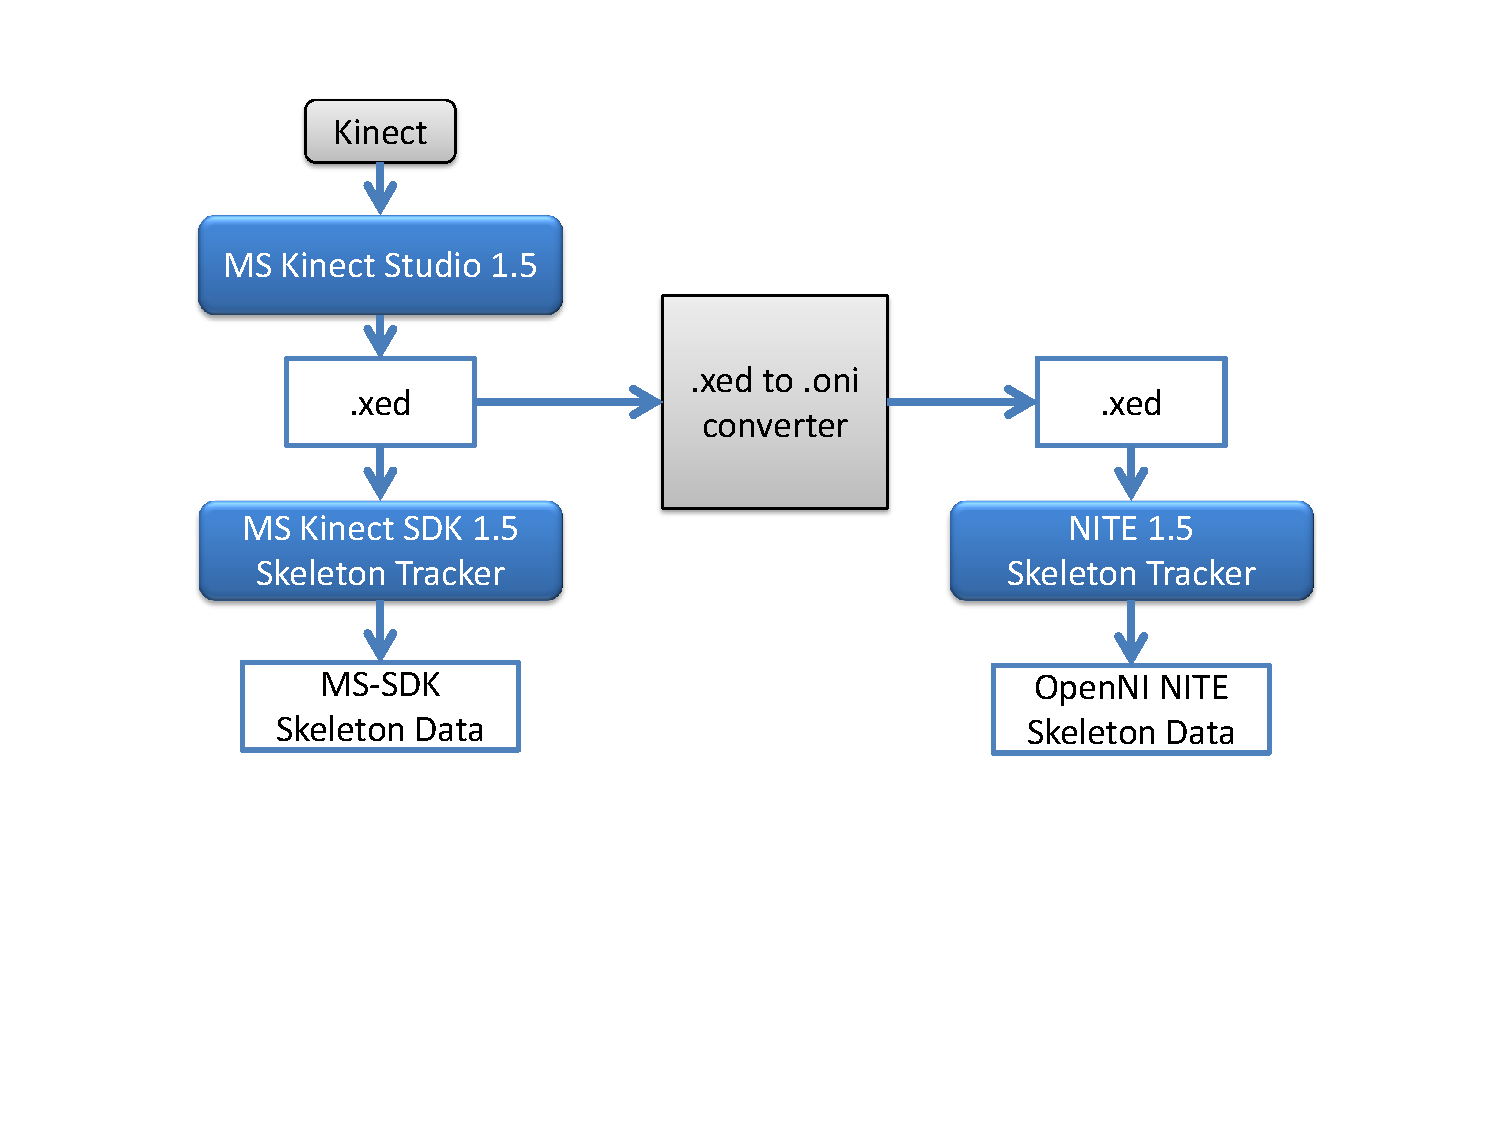
\includegraphics[width=0.75\textwidth]{pics/xedoni_2_cropped}
\caption{Data capturing pipeline for error analysis.}
\label{fig:xedoni}
\end{figure}

In order to be able to do a fair comparison between MS-SDK and OpenNI skeleton trackers, we used the same dataset for both. MS-SDK and OpenNI use different device drivers, therefore can not be directly used on the live depth stream at the same time. Because of this, we extract the skeleton data offline in multiple stages. The pipeline for the data capture procedure is illustrated in Figure \ref{fig:xedoni}. We first save the depth streams as .xed files using Microsoft Kinect Studio program. The acquired .xed file is converted to .oni in a OpenNI recorder application by streaming the depth stream to through Kinect Studio. The .oni is then played back in skeleton tracking application in OpenNI, which writes the OpenNI skeleton data to a .txt file. MS-SDK skeleton data is obtained by playing back the original .xed in the skeleton tracking application.

%\subsection{Pointing Gesture Annotation}
%\label{sec:pointing_gesture_annotation}

To factor out the effectiveness of our pointing gesture recognition method described in Section \ref{sec:pointing_pointing_gesture_recognition}, we manually started the time when each pointing gesture began for data collection. Starting from the onset of the pointing gesture as annotated by the experimenter, the following $30$ sensor frames were used as the pointing gesture. This corresponds to a recording of $1$ second in the Kinect sensor stream. For each frame, we extracted skeleton data using both the MS-SDK and the OpenNI.

\subsection{Evaluation}
\label{sec:pointing_evaluation}


\subsubsection{Error Analysis}
\label{sec:pointing_error_analysis}

The four rays corresponding to the four different pointing approaches described in Section \ref{sec:pointing_pointing_gesture_recognition} were used for our error analysis.  As described in Section \ref{sec:ground_truth_points}, the ground truth target positions are available. We computed two types of errors for each gesture and target:

\begin{itemize}
\item Euclidean error of ray intersections with target planes (Figure \ref{fig:euclidean_projections})
\item Angular error in spherical coordinates (Tables \ref{table:pointing_horizontal}, \ref{table:pointing_vertical} and Figure \ref{fig:pointing_angular_boxplots})
\end{itemize}

We elaborate our error analysis subsequent sections.

\begin{landscape}
\begin{figure}[t!]
\centering
\vspace*{-1.0cm}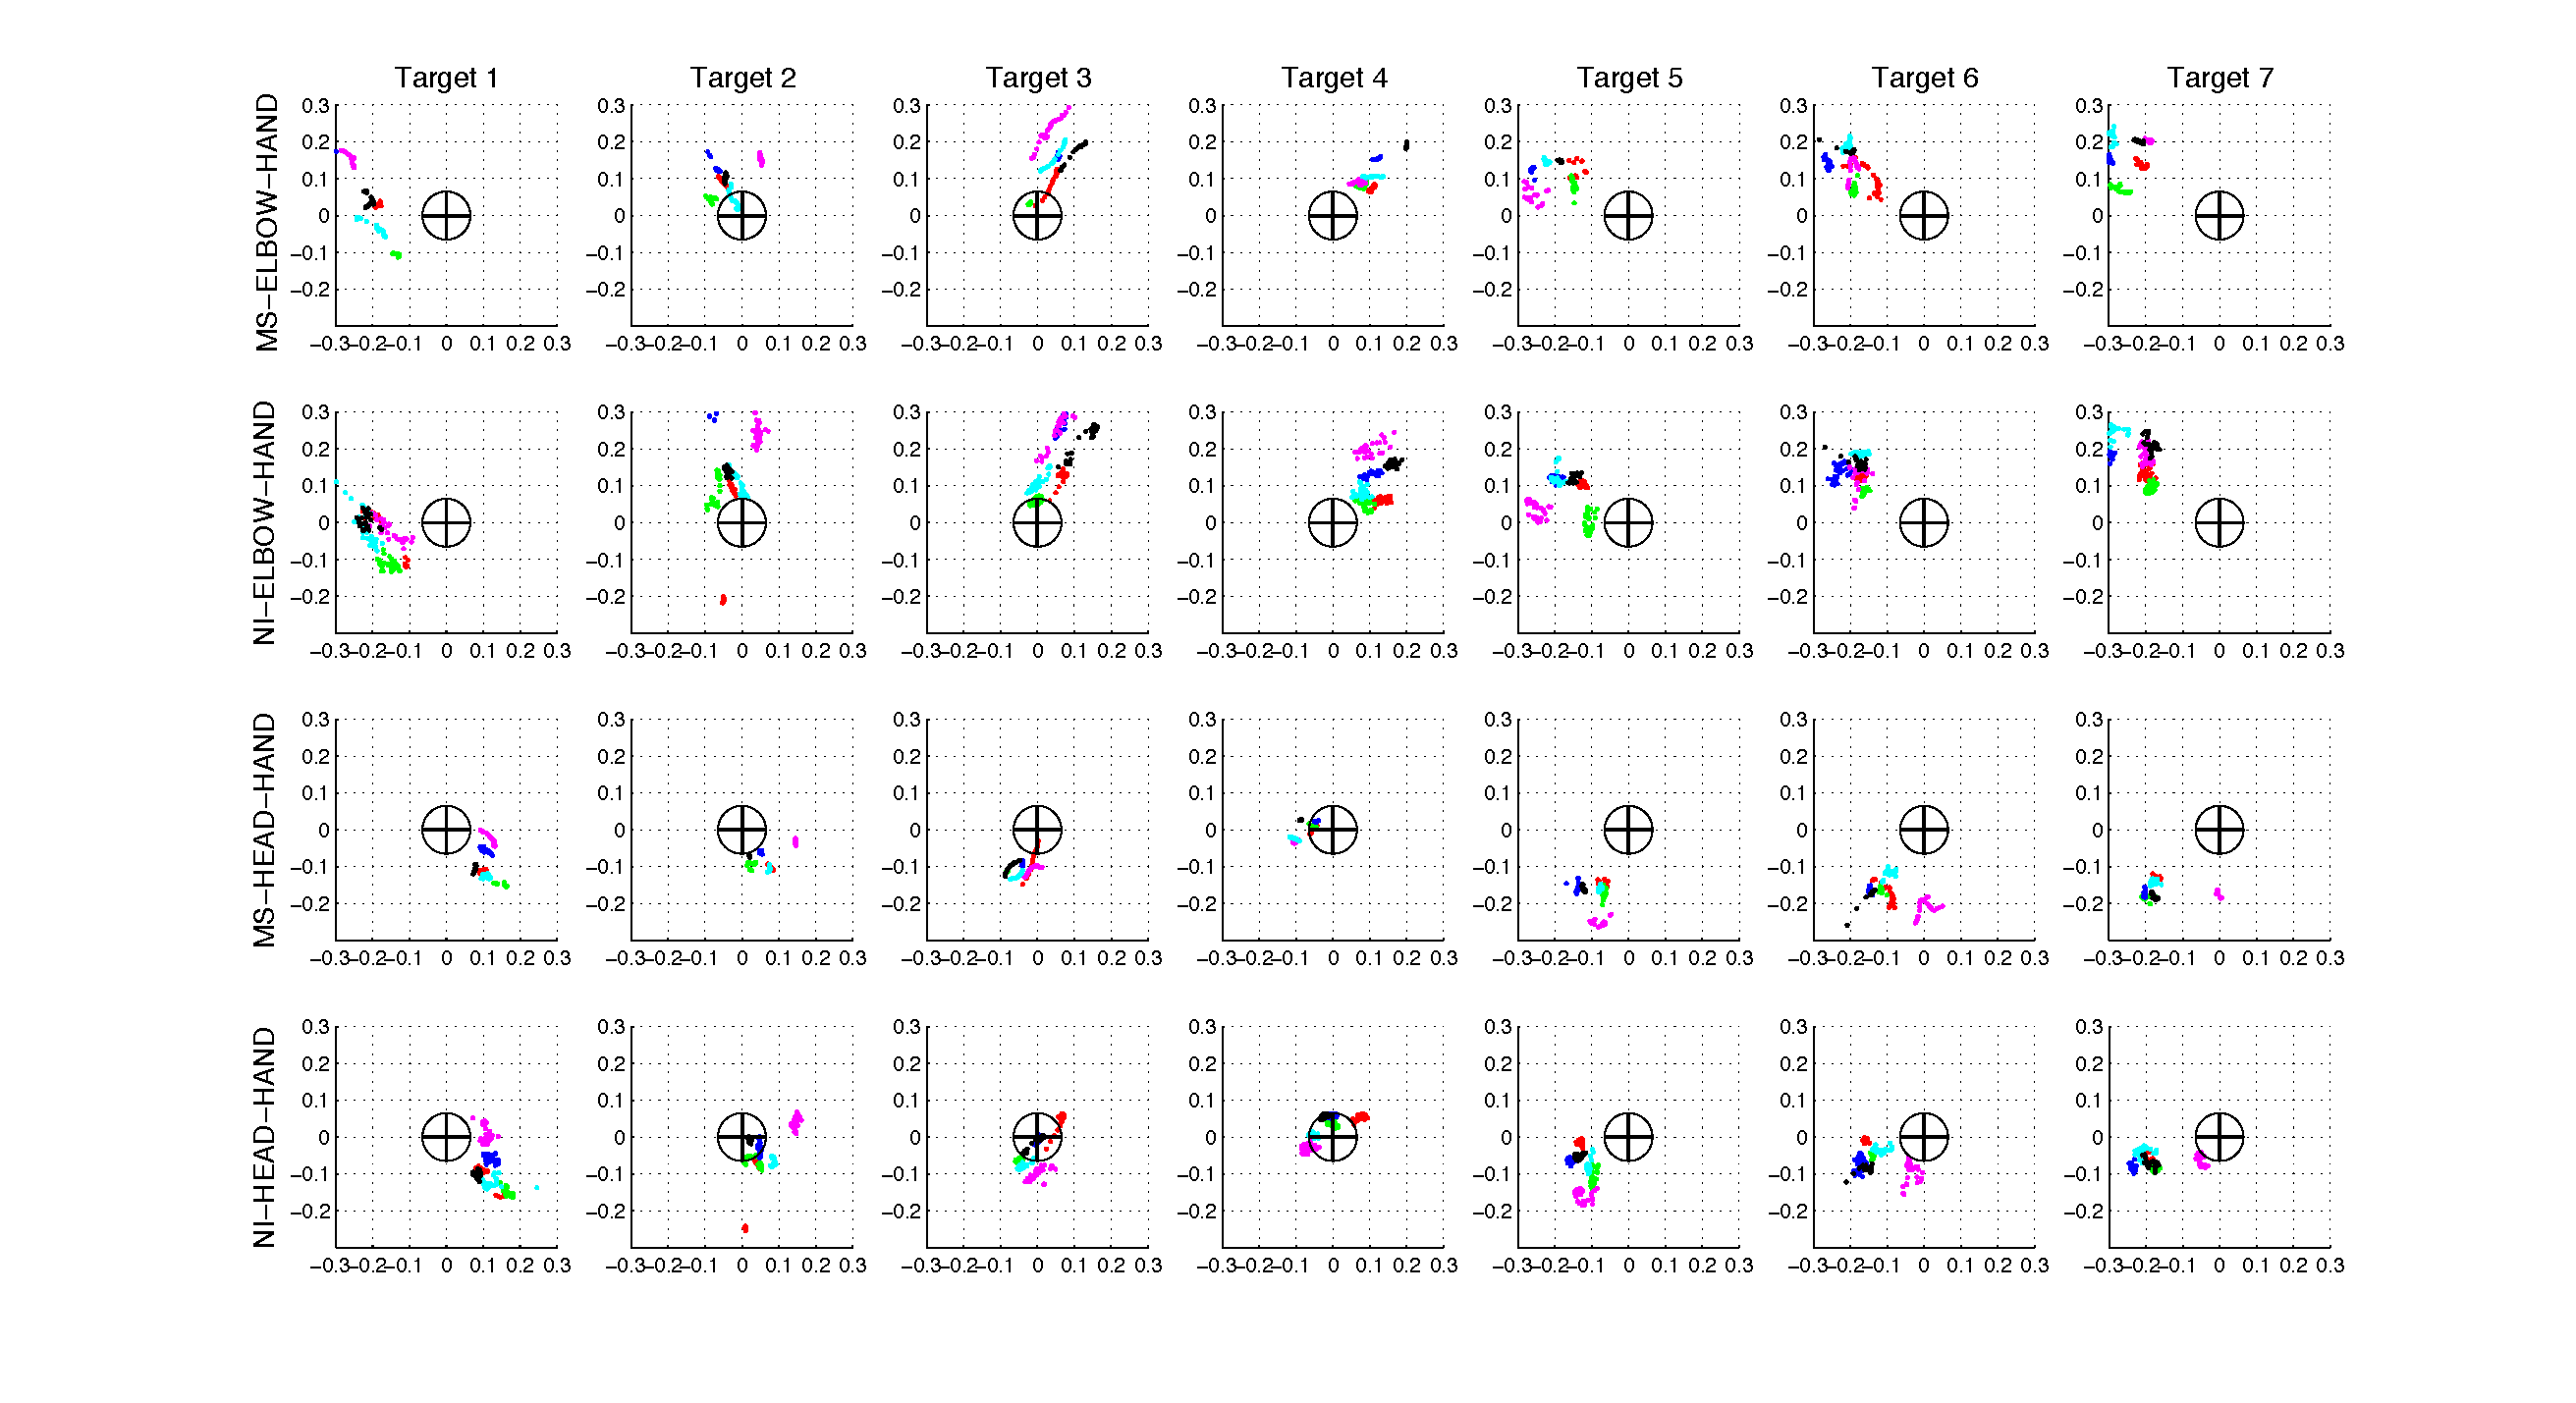
\includegraphics[width=1.5\textwidth]{pics/projections.pdf}
\caption{(Best viewed in color). Euclidean distance error in cartesian coordinates for each gesture method and target. The pointing ray intersection points with the target plane are shown here for each target (T1-T7) as the columns.  Each subject's points are shown in separate colors.  There are 30 points from each subject, corresponding to the 30 frames recorded for the pointing gesture at each target.  Axes are shown in centimeters.  The circle drawn in the center of each plot has the same diameter (13 cm) as the physical target objects used.}
\label{fig:euclidean_projections}
\end{figure}
\end{landscape}

\begin{landscape}% Landscape page

\begin{center}

\begin{table*}
\caption{$\mu$ and $\sigma$ angular errors in degrees for each of Targets 1-4 (Figure \ref{fig:ground_truth_targets}), for each pointing method. The aggregate $\mu$ and $\sigma$ is also shown.}
\centering
\begin{tabular}{c| @{} x{1.0cm}| @{} x{1.0cm}| @{} x{1.0cm}| @{} x{1.0cm}| @{} x{1.0cm}| @{} x{1.0cm}| @{} x{1.0cm}| @{} x{1.0cm}| @{} x{1.0cm}| @{} x{1.0cm}| @{} x{1.0cm}| @{} x{1.0cm}| @{} x{1.0cm}| @{} x{1.0cm}| @{} x{1.0cm}| @{} p{1.0cm}|}
\cline{2-17}
& \multicolumn{4}{c|}{Target 1} & \multicolumn{4}{c|}{Target 2} & \multicolumn{4}{c|}{Target 3} & \multicolumn{4}{c|}{Target 4} \\ \cline{2-17}
& \multicolumn{2}{c|}{$\theta$} & \multicolumn{2}{c|}{$\psi$} & \multicolumn{2}{c|}{$\theta$} & \multicolumn{2}{c|}{$\psi$}  & \multicolumn{2}{c|}{$\theta$} & \multicolumn{2}{c|}{$\psi$}  & \multicolumn{2}{c|}{$\theta$} & \multicolumn{2}{c|}{$\psi$}\\ \cline{2-17}
& \footnotesize{$\mu$} & \footnotesize{$\sigma$} & \footnotesize{$\mu$} & \footnotesize{$\sigma$} & \footnotesize{$\mu$} & \footnotesize{$\sigma$} & \footnotesize{$\mu$} & \footnotesize{$\sigma$} & \footnotesize{$\mu$} & \footnotesize{$\sigma$} & \footnotesize{$\mu$} & \footnotesize{$\sigma$} & \footnotesize{$\mu$} & \footnotesize{$\sigma$} & \footnotesize{$\mu$} & \footnotesize{$\sigma$} \\ \hline
\multicolumn{1}{ |c|}{\textbf{\scriptsize{MS-Elbow-Hand}}}& -15.7 & 2.9  & 5.5 & 6.1  & -4.3 & 6.6  & 7.8 & 3.1  & -3.7 & 2.4  & 7.4     & 3.1  & -3.6 & 1.9  & 11.5 &\multicolumn{1}{r|}{2.9}\\ \hline
\multicolumn{1}{ |c|}{\textbf{\scriptsize{NI-Elbow-Hand}}}& -16.4 & 2.9  & 4.3 & 7.0  &  -3.8 & 6.6  & 11.3 & 10.9  & -4.8 & 2.6  & 9.7 & 3.4  & -4.0 & 4.7  & 12.4 &\multicolumn{1}{r|}{2.5} \\ \hline
\multicolumn{1}{ |c|}{\textbf{\scriptsize{MS-Head-Hand}}}& 7.7 & 2.6  & -12.0 & 5.3  & 10.8 & 6.4  & -9.1 & 3.2  & 2.2 & 2.0 & -8.3   & 3.2  & -4.0 & 1.7  & -4.3 &\multicolumn{1}{r|}{3.2} \\ \hline
\multicolumn{1}{ |c|}{\textbf{\scriptsize{NI-Head-Hand}}}& 8.5 & 2.6 & -11.7 & 6.1  & 10.2 & 6.7  & -5.7 & 8.0  & 2.0 & 2.3  & -2.9    & 4.7  & -3.2 & 2.5  & 1.45 &\multicolumn{1}{r|}{4.8} \\ \hline
\end{tabular}
\label{table:pointing_horizontal}
\end{table*}

\vspace*{\fill}

\begin{table*}
\caption{$\mu$ and $\sigma$ of angular error in degrees for each of Targets 5-7 (Figure \ref{fig:ground_truth_targets}), for each pointing method. The aggregate $\mu$ and $\sigma$ is also shown.}
\centering
\begin{tabular}{c| @{} x{1.0cm}| @{} x{1.0cm}| @{} x{1.0cm}| @{} x{1.0cm}| @{} x{1.0cm}| @{} x{1.0cm}| @{} x{1.0cm}| @{} x{1.0cm}| @{} x{1.0cm}| @{} x{1.0cm}| @{} x{1.0cm}| @{} x{1.0cm}| @{} x{1.0cm}| @{} x{1.0cm}| @{} x{1.0cm}| @{} p{1.0cm}|}
\cline{2-17}
& \multicolumn{4}{c|}{Target 5} & \multicolumn{4}{c|}{Target 6} & \multicolumn{4}{c|}{Target 7} & \multicolumn{4}{c|}{ALL TARGETS} \\ \cline{2-17}
& \multicolumn{2}{c|}{$\theta$} & \multicolumn{2}{c|}{$\psi$} & \multicolumn{2}{c|}{$\theta$} & \multicolumn{2}{c|}{$\psi$}  & \multicolumn{2}{c|}{$\theta$} & \multicolumn{2}{c|}{$\psi$}  & \multicolumn{2}{c|}{$\theta$} & \multicolumn{2}{c|}{$\psi$}\\ \cline{2-17}
& \footnotesize{$\mu$} & \footnotesize{$\sigma$} & \footnotesize{$\mu$} & \footnotesize{$\sigma$} & \footnotesize{$\mu$} & \footnotesize{$\sigma$} & \footnotesize{$\mu$} & \footnotesize{$\sigma$} & \footnotesize{$\mu$} & \footnotesize{$\sigma$} & \footnotesize{$\mu$} & \footnotesize{$\sigma$} & \footnotesize{$\mu$} & \footnotesize{$\sigma$} & \footnotesize{$\mu$} & \footnotesize{$\sigma$} \\ \hline
\multicolumn{1}{ |c|}{\textbf{\scriptsize{MS-Elbow-Hand}}}& -14.5 & 4.1  & 11.6 & 3.7  & -16.6 & 3.3  & 9.9 & 3.7  & -20.8 & 3.7  & 5.7 & 3.4  & -11.3 & 7.7  & 8.5 &\multicolumn{1}{r|}{4.5}\\ \hline
\multicolumn{1}{ |c|}{\textbf{\scriptsize{NI-Elbow-Hand}}}& -12.9 & 4.2  & 9.7 & 5.1  & -16.2 & 2.6  & 11.7 & 3.7  & -20.2 & 4.5  & 8.1 & -3.0  & -11.2 & 7.6  & 9.6 &\multicolumn{1}{r|}{6.3} \\ \hline
\multicolumn{1}{ |c|}{\textbf{\scriptsize{MS-Head-Hand}}}& -9.4 & 1.9  & -11.6 & 3.0  & -7.1 & 4.7  & -13.8 & 1.8  & -8.0 & 5.5 & -15.6 & -2.9  & -1.1 & 8.5  & -10.7 &\multicolumn{1}{r|}{4.8} \\ \hline
\multicolumn{1}{ |c|}{\textbf{\scriptsize{NI-Head-Hand}}}& -11.5 & 1.5 & -4.7 & 4.8  & -11.2 & 4.8  & -4.9 & 2.9  & -12.3 & 5.2  & -8.9 & -2.5  & -2.4 & 9.6  & -5.3 &\multicolumn{1}{r|}{6.4} \\ \hline
\end{tabular}

\label{table:pointing_vertical}
\end{table*}

\end{center}
\end{landscape}


\subsubsection{Euclidean error}
\label{sec:pointing_euclidean_error}

Given a ray $\vec{v}$ in the sensors frame from one of the pointing gesture approaches, and a ground truth target point $p_{target}$ lying on a target planar surface, the ray-plane intersection between $\vec{v}$ and plane was computed for each ray, resulting in a 3D point lying on the plane. Figure \ref{fig:euclidean_projections} shows the 2D projections for all 30 measurements from each subject (shown in different colors) and each target. For ease of display, the 3D intersection coordinates with the target planes are displayed in a 2D coordinate system attached to the target plane, with the ground truth target point as the origin.  

As can be seen in Figure \ref{fig:euclidean_projections},  the pointing gesture intersection points were fairly consistent across all users, but varied per target location.  The elbow-hand method produced similar results for MS-SDK and OpenNI. The same is true for the head-hand method.  It is also noteworthy that the data for each target tends to be quite clustered for all methods, and typically not centered on the target location.

\subsubsection{Angular Error}
\label{sec:pointing_angular_error}

We computed the mean and standard deviations of the angular errors in the spherical coordinate system for each pointing gesture method and target. Section \ref{sec:pointing_representing_pointing_directions} describes in detail how the angles $(\theta, \psi)$ are found. The mean and standard deviation values are given in Tables \ref{table:pointing_horizontal} and \ref{table:pointing_vertical}.  The aggregate errors are also displayed as a  box plot in Figure \ref{fig:pointing_angular_boxplots}.

Several observations can be made from these results. The data from the elbow-hand pointing method reports that users typically point about 11 degrees to the left of the intended target direction, and about 9 above the target direction. Similarly, the data from the head-hand pointing method reports that users typically point about 2 degrees to the left of the intended pointing direction, but with a higher standard deviation than the elbow-hand method.  On average, the vertical angle $\psi$ was about 5 degrees below the intended direction for the OpenNI tracker and 10 degrees below for the MS-SDK tracker, with a higher standard deviation than the elbow-hand methods.  The disparity between the two skeleton trackers for this pointing method is because they report different points for the head position, with the MS-SDK head position typically being reported higher than the OpenNI head position. The overall performance of the OpenNI and MS-SDK skeleton trackers, however, is fairly similar, with the MS-SDK having slightly less variation for our dataset.

\begin{figure*}[ht!]%[thpb]
\centering
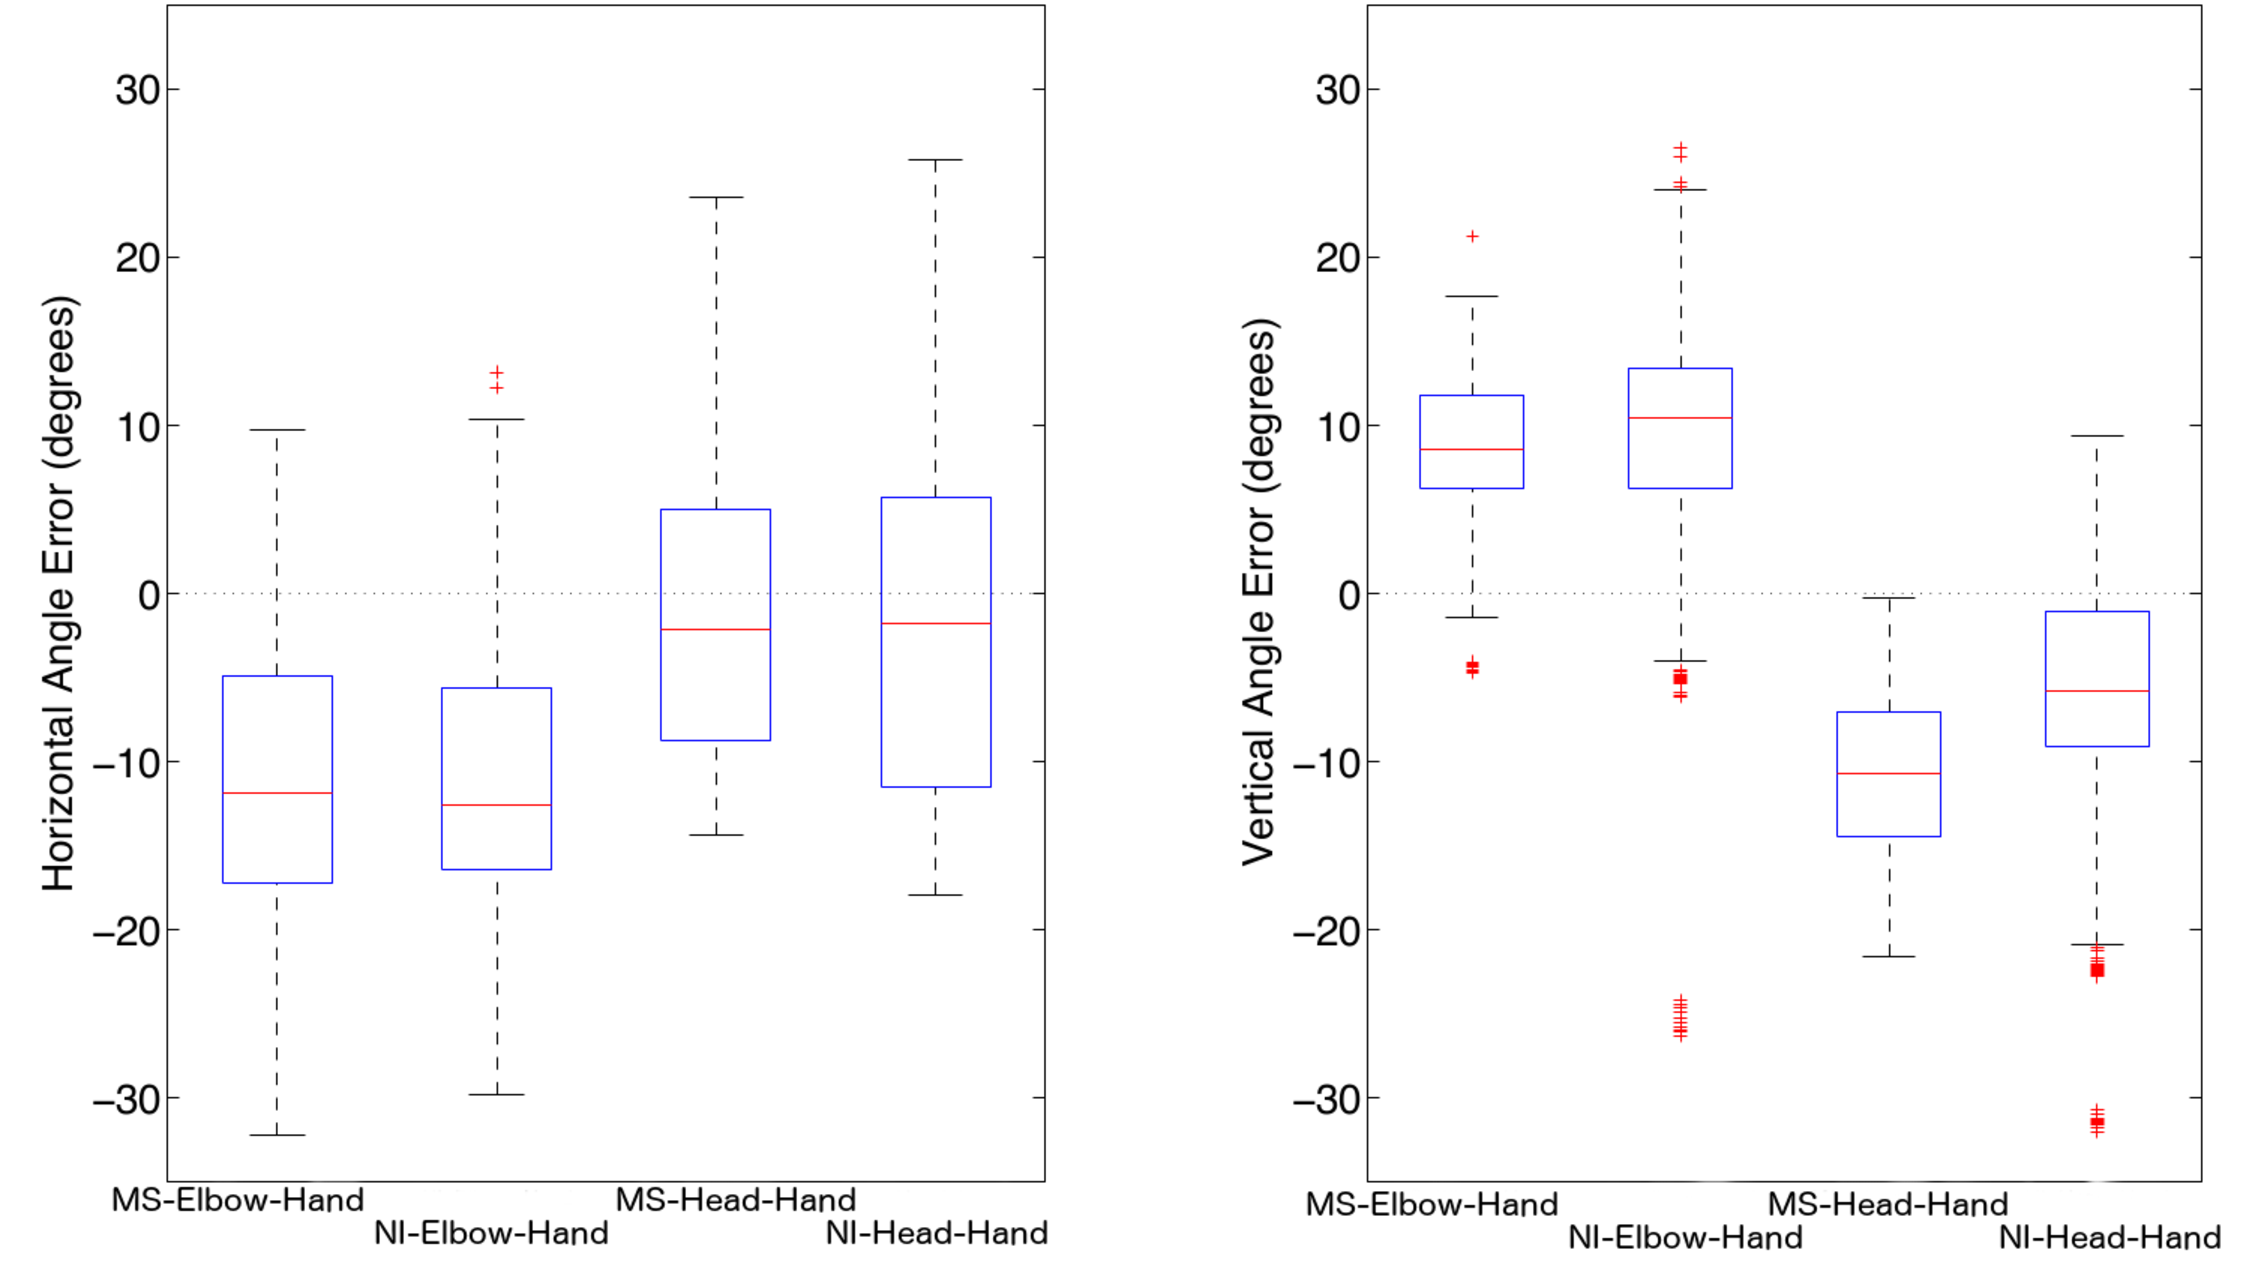
\includegraphics[width=1.0\textwidth]{pics/boxplots_largerfont}
\caption{Box plots of the errors in spherical coordinates $\theta$ and $\psi$ for each pointing method.}
\label{fig:pointing_angular_boxplots}
\end{figure*}

As can be seen in the aggregate box plot in Figure \ref{fig:pointing_angular_boxplots}, the horizontal angle $\theta$ has a higher variation than the vertical angle $\psi$.  Examining the errors for individual target locations shows that this error changes significantly with the target location.  As future work, it would be interesting to collect data for a higher density of target locations to attempt to parameterize any angular correction that might be applied.



\subsubsection{Object Separation Analysis}

%\subsection{Evaluation}
%\label{sec:pointing_evaluation}

Using the error analysis and pointing gesture model we presented in previous sections, we conducted an experiment to  determine how our approach distinguished two potentially ambiguous pointing target objects. We use the results of the angular error analysis results and not the euclidean error analysis for the remainder of the paper because of our angular representation of pointing gestures.

\begin{figure}[ht!]
\centering
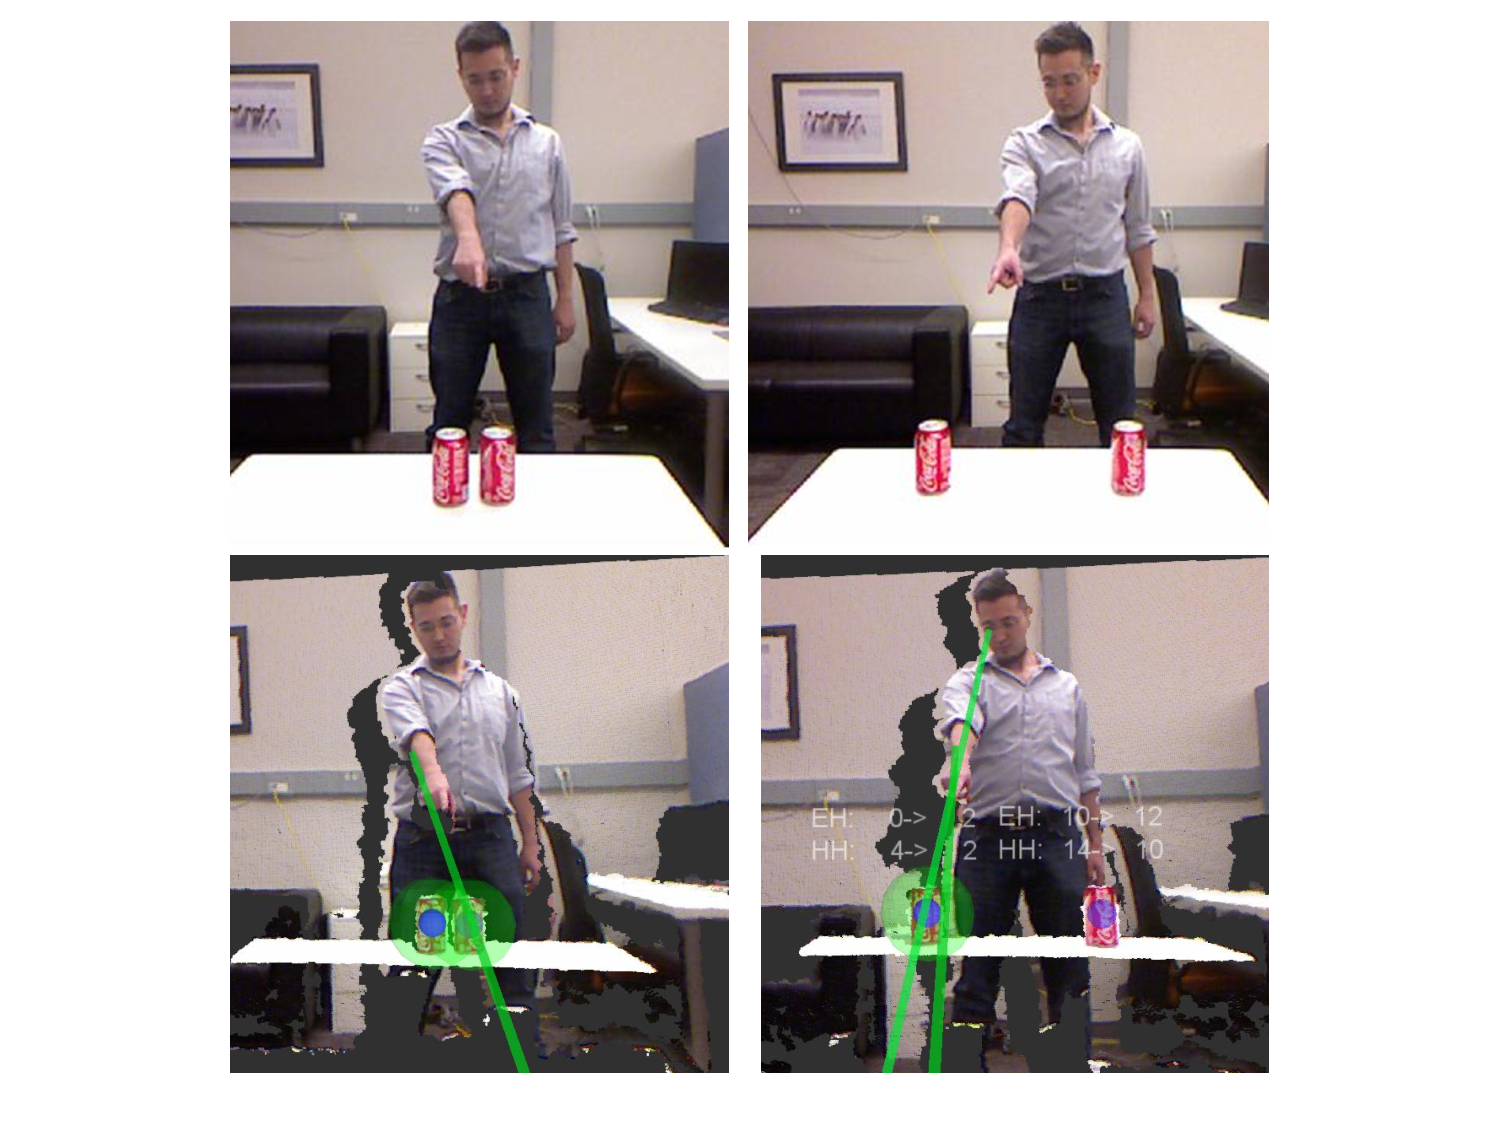
\includegraphics[width=0.75\textwidth]{pics/separation_2_cropped}
\caption{Example scenarios from the object separation test is shown. Our experiments covered separations between 2cm (left images) and 30cm (right images). The object is comfortably distinguished for the 30cm case, whereas the intended target is ambiguous when the targets are 2cm apart. Second row shows the point cloud from Kinect's view. Green lines show the Elbow-Hand and Head-Hand directions whereas green circles show the objects that are within the threshold $D_{mah}<2$.}
\label{fig:pointing_separation}
\end{figure}


The setup consisted of a table between the robot and the person and two coke cans on the table (Figure~\ref{fig:pointing_separation}) where the separation between objects was varied. To detect the table plane and segment out the objects on top of it, we used the segmentation approach presented in~\cite{trevor2013segmentation}. The objects centroid positions, along with their point clouds were calculated in real-time using our segmentation algorithm. The separation between objects were varied with 1 cm increments from $2-15cm$ and with $5cm$ increments between $15-30 cm$. We could not conduct the experiment below 2 cm separation because of the limitations of our perception system. We used the OpenNI skeleton tracker because rest of our system is based in Linux, and we already found that performance difference with MS-SDK for pointing angle errors is insignificant. The experiment was conducted with one user, who was not in the training dataset. For each separation, the user performed 5 pointing gestures to the object on the right and 5 to the object on the left. The person pointed to one of the objects and the Mahalanobis distance $D_{mah}$ to the intended object and the other object is calculated using the approach in Section \ref{sec:pointing_determining_intended_target}. We used the mean and standard deviation values of Target 2 (Figure \ref{fig:ground_truth_targets}) for this experiment because the objects were located between the robot and the person.


\begin{figure*}[ht!]
\centering
%
        \subfigure[]{%
            \label{fig:eh_graph}
            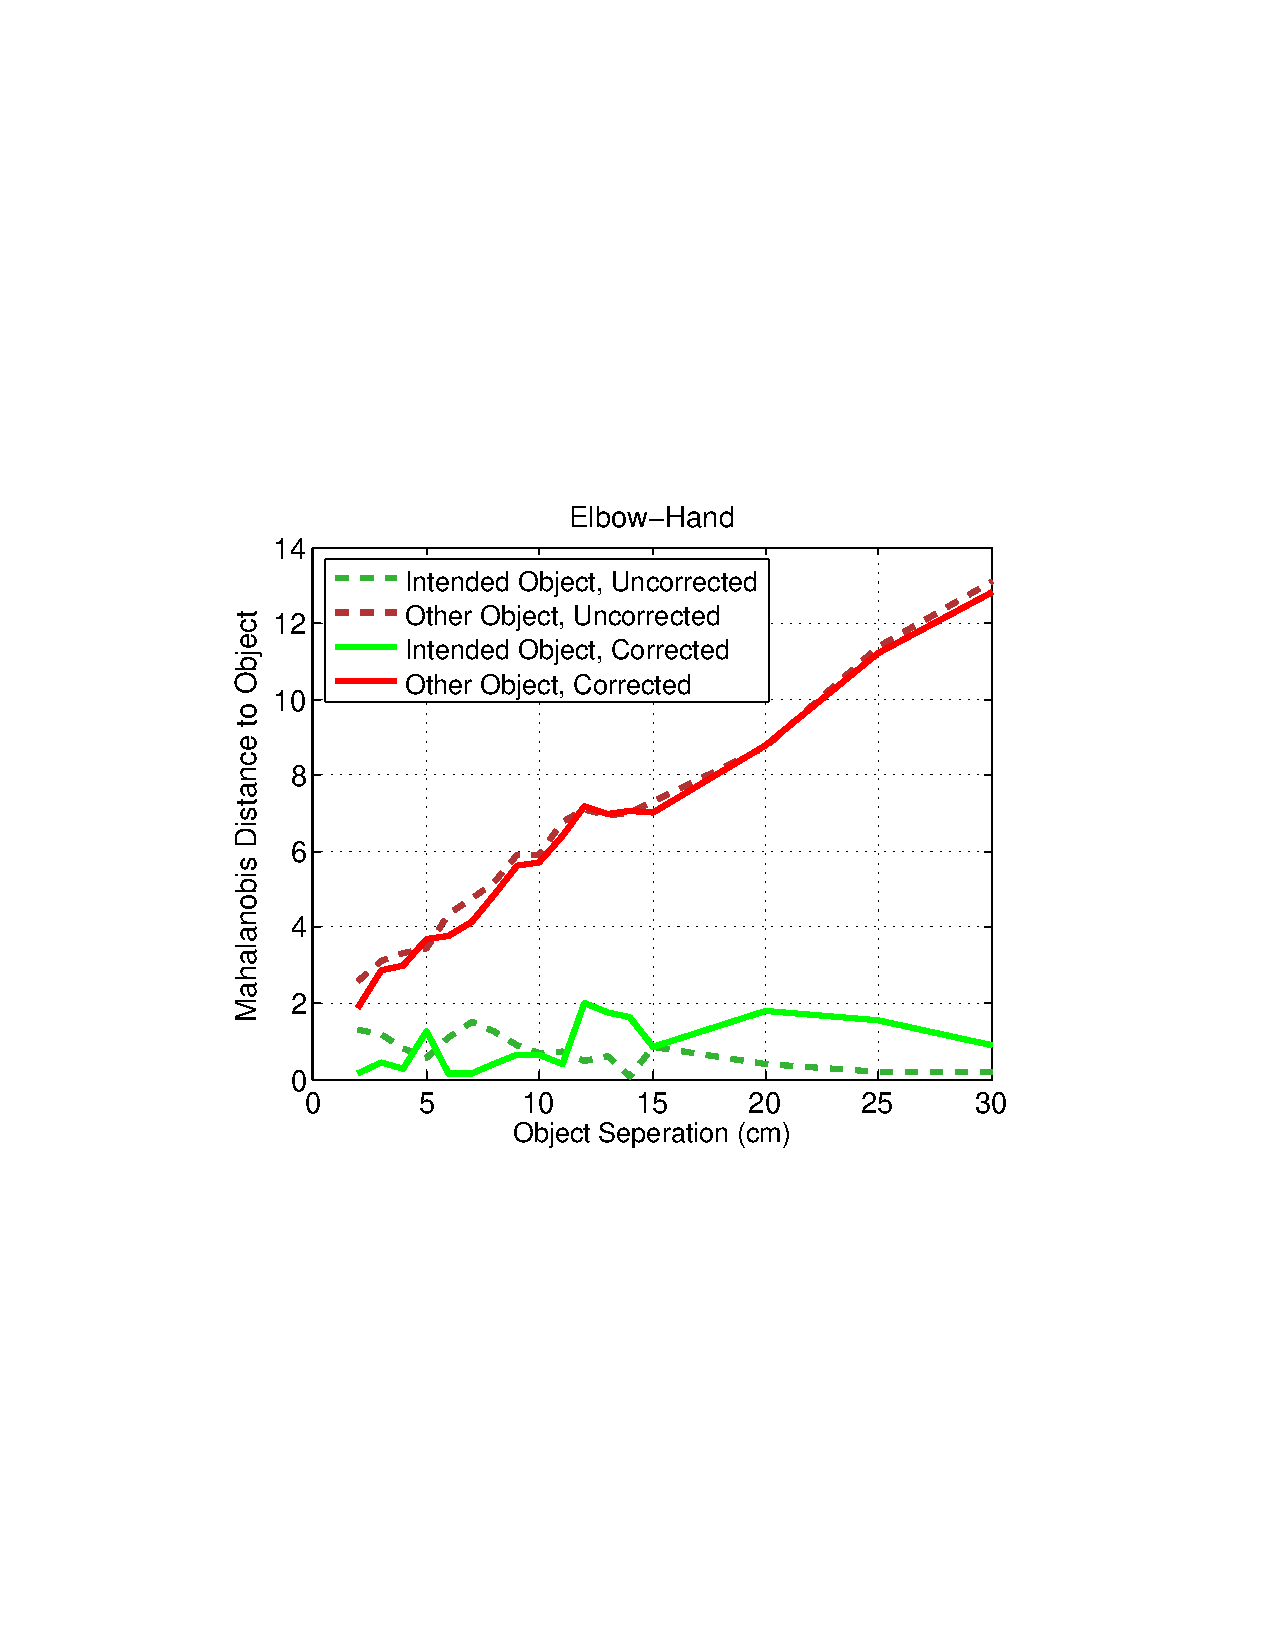
\includegraphics[width=73mm]{pics/eh_graph_crop}
        }%
        \subfigure[]{%
           \label{fig:hh_graph}
           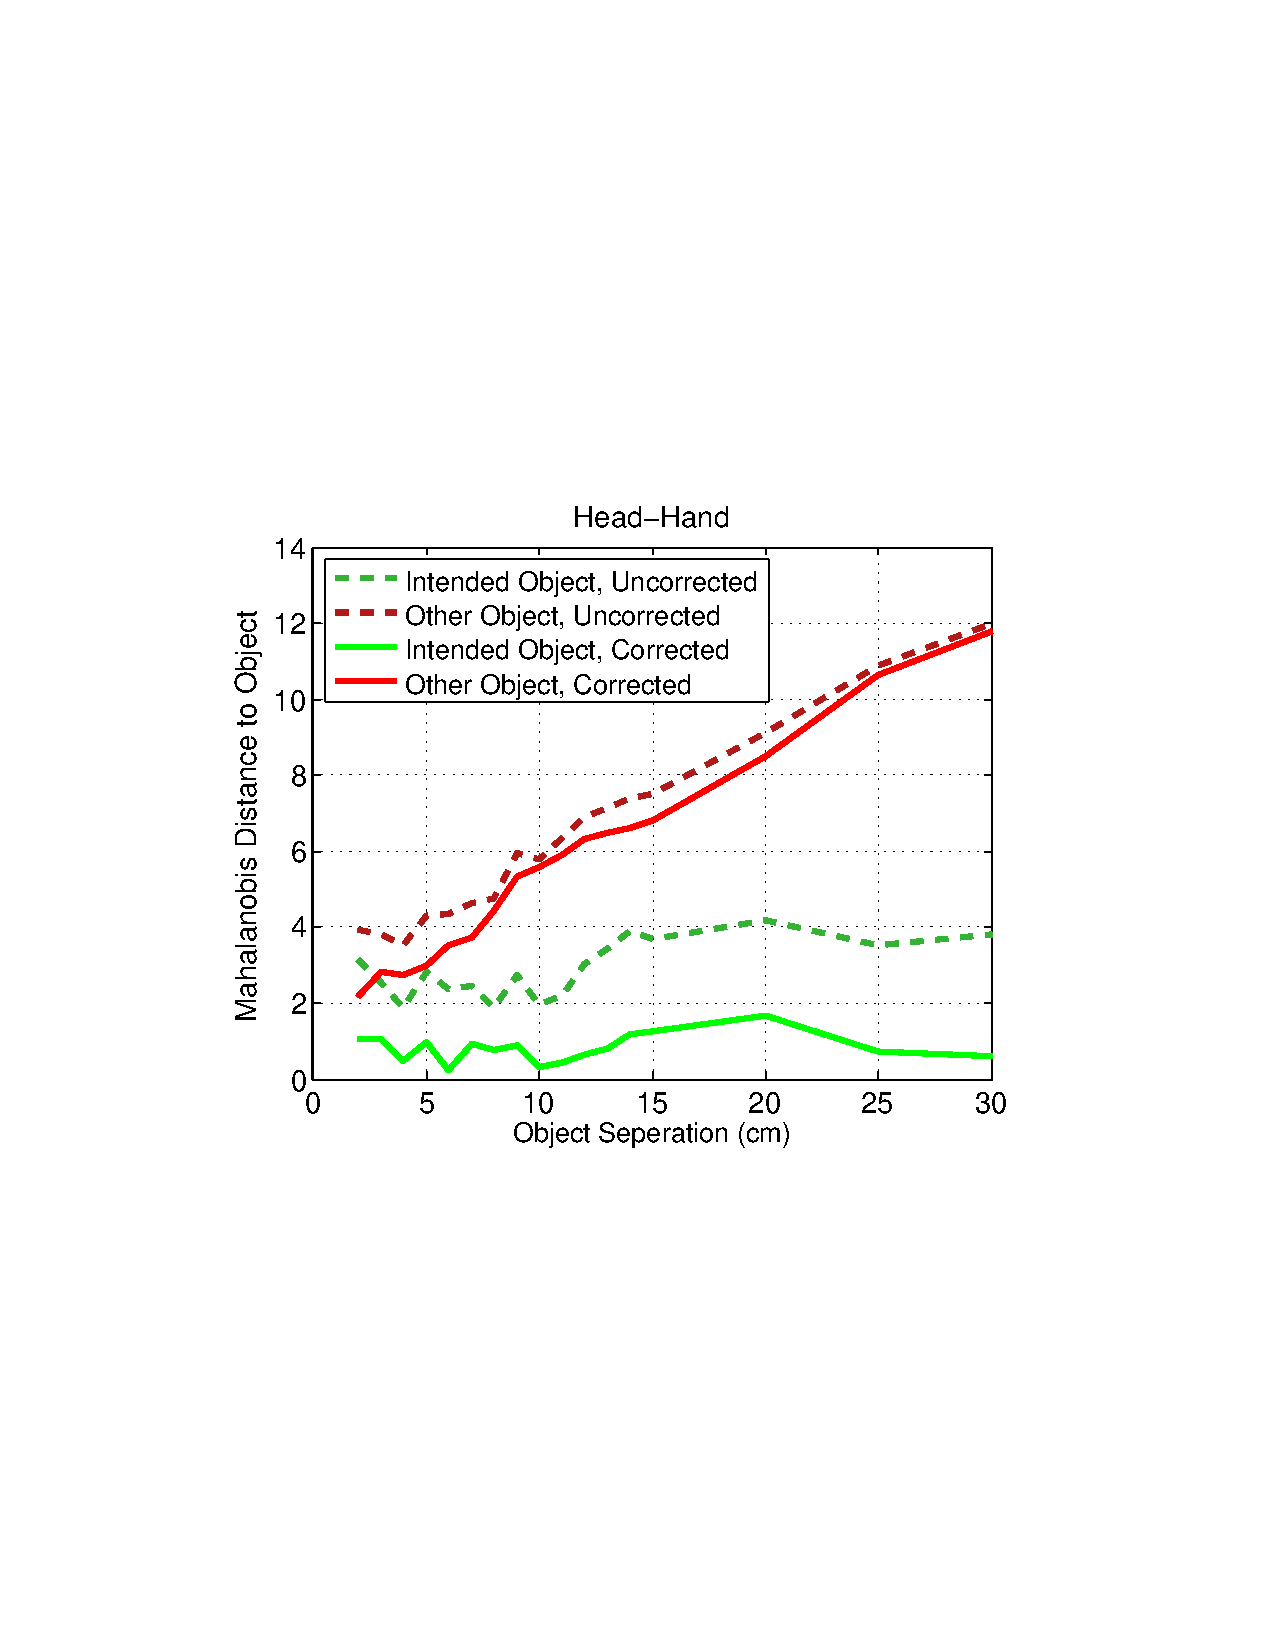
\includegraphics[width=73mm]{pics/hh_graph_crop}
        }        
    \caption{%
	Resulting Mahalanabis distances of pointing targets from the Object Separation Test is shown for a) Elbow-Hand and b) Head-Hand pointing methods. Intended object are shown in green and other object is in red. Solid lines show distances after correction is applied. Less Mahalanobis distance for intended object is better for reducing ambiguity.
     }%
   \label{fig:pointing_graphs}
\end{figure*}

\subsubsection{Results and Discussion}
\label{sec:results_and_discussion}

The results of the object separation experiment is given for Elbow-Hand (Figure~\ref{fig:eh_graph}) and Head-Hand (Figure~\ref{fig:hh_graph}) methods. The graphs plot object separation versus the Mahalanobis distance for the pointed object and the other object for corrected and uncorrected pointing direction. There are several observations we make by looking at these results.

First, the Mahalanobis distance $D_{mah}$ for the intended object was always lower than the other object. The corrected $D_{mah}$ for both Elbow-Hand and Head-Hand methods for the intended object was always below 2, therefore selecting the threshold $D_{thres}=2$ is a reasonable choice. We notice that some distances for the unintended object at $2cm$ separation is also below $D_{mah}<2$. Therefore, when the objects are $2 cm$ apart, then the pointing target becomes ambiguous for this setup. For separations of $3cm$ or more, $D_{mah}$ of the unintended object is always over the threshold, therefore there is no ambiguity.

Second, correction significantly improved Head-Hand accuracy at all separations, slightly improved Elbow-Hand between $2-12cm$ but slightly worsened Elbow-Hand after $12cm$. We attribute this to the fact that the angles we receive is heavily user-dependent and can have a significant variance across methods as showed in Figure~\ref{fig:pointing_angular_boxplots}. Moreover, the user was not in the training set.

Third, the Mahalanobis distance stayed generally constant for the intended object, which was expected. It linearly increased with separation distance for the other object.

Fourth, patterns for both methods are fairly similar to each other, other than Head-Hand uncorrected distances being higher than Elbow-Hand.

\subsubsection{Conclusions}
\label{sec:pointing_conclusions}

Humans and robots engaged in joint actions that involve objects will need to be able to communicate about these objects. Deictic gestures can play a crucial part such communication, especially when establishing goals and negotiating responsibilities. A pointing target detection approach that returns a single hypothesis can lead to failures due to perception error. On the other hand, estimation of a pointing likelihood of nearby objects can give valuable insight to a robot. For example, a robot can ask the user to disambiguate the objects if it perceives more than one object that has a significant likelihood of being referred to.

In this work, we model the uncertainty of pointing gestures in a spherical coordinate system, use this model to determine the correct pointing target, and detect when there is ambiguity. Two pointing methods are evaluated using two skeleton tracking algorithms: Elbow-Hand and Head-Hand rays, using both OpenNI NITE and Microsoft Kinect SDK.  A data collection with 6 users and 7 pointing targets was performed, and the data was used to model users pointing behavior.  The resulting model was evaluated for its ability to distinguish between potential pointing targets, and to detect when the target is ambiguous. Our evaluation showed that in a scenario where the separation between two objects were varied, our system was able to identify that there is ambiguity for 2 cm separation and comfortably distinguished the intended object for 3 cm or more separation.
